
In the previous lectures we considered multi-stage decision problems for \emph{deterministic} systems. In many problems of interest, the system dynamics also involve \emph{randomness}, which leads us to stochastic decision problems. In this chapter we introduce the basic model of Markov Decision Processes, which will be considered is the rest of the course.
%Contents:
%4.1  Markov Chains (Reminder)
%4.2  Controlled Markov Chains
%4.3  Performance Criteria
%4.4 * Sufficiency of Markov policies
%4.4  Finite-horizon Dynamic Programming  (reading assignment)
%
%Note: Corrections (in red) on pages: 2, 3, 7, 13, 16

\section{Markov Chains: A Reminder}

A Markov chain $\{ {X_t},\;t = 0,1,2, \ldots \} $, with ${X_t} \in X$, is a discrete-time stochastic process, over a finite or countable state-space $X$, that satisfies the following Markov property:
	\[{\cal P}({X_{t + 1}} = j|{X_t} = i,{X_{t - 1}}, \ldots {X_0}) = {\cal P}({X_{t + 1}} = j|{X_t} = i).\]
We focus on time-homogeneous Markov chains, where
\[{\cal P}({X_{t + 1}} = j|{X_t} = i) = {\cal P}({X_1} = j|{X_0} = i) \buildrel \Delta \over = {p_{ij}}.\]
The ${p_{ij}}$'s  are the transition probabilities, which satisfy
${p_{ij}} \ge 0,\;\;\;\sum\nolimits_{j \in X} {{p_{ij}} = 1\;\;\forall i} $.
The matrix $P = ({p_{ij}})$ is the transition matrix.

Given the initial distribution ${p_0}$ of ${X_0}$, namely $p({X_0} = i) = {p_0}(i)$, we obtain the finite-dimensional distributions:
\[{\cal P}({X_0} = {i_0}, \ldots ,{X_t} = {i_t}) = {p_0}(i_0){p_{{i_0}{i_1}}} \cdot  \ldots  \cdot {p_{{i_{t - 1}}{i_t}}}.\]

Define $p_{ij}^{(m)} = {\cal P}({X_m} = j|{X_0} = i),$ the m-step transition probabilities.  It is easy to verify that $p_{ij}^{(m)} = {[{P^m}]_{ij}}$  (here ${P^m}$ is the m-th power of the matrix $P$).

\paragraph{State classification:}
\begin{itemize}
\item State $j$ is accessible from $i$  ($i \to j$) if $p_{ij}^{(m)} > 0$ for some $m \ge 1$.
\item $i$ and $j$ are communicating states (or communicate) if $i \to j$ and $j \to i$.
\item A communicating class (or just class) is a maximal collection of states that communicate.
\item The Markov chain is irreducible if all states belong to a single class (i.e., all states communicate with each other).
\item State $i$ is periodic with period $d \ge 2$ if  $p_{ii}^{(m)} = 0$ for $m \ne \ell d$ and  $p_{ii}^{(m)} > 0$ for $m = \ell d$, $\ell \in \{ 1,2, \ldots \}$. Periodicity is a class property: all states in the same class have the same period.
\end{itemize}

\paragraph{Recurrence:}
\begin{itemize}
\item State $i$ is recurrent if ${\cal P}({X_t} = i{ \textrm{ for some }}t \ge 1|{X_0} = i) = 1$. Otherwise, $i$ is transient.
\item State $i$ is recurrent if and only if $\sum\nolimits_{m = 1}^\infty  {p_{ii}^{(m)}}  = \infty $.
\item Recurrence is a class property.
\item If $i$ and $j$ are in the same recurrent class, then $j$ is (eventually) reached from $i$ with probability 1:  ${\cal P}({X_t} = j{\textrm{ for some t}} \ge 1|{X_0} = i) = 1$.
\item Let ${T_i}$ be the return time to state $i$  (number of stages required for $({X_t})$ to return to $i$). If $i$ is a recurrent state, then ${T_i} < \infty $ w.p. 1.
\item State $i$ is positive recurrent if  $E({T_i}) < \infty $, and null recurrent if $E({T_i}) = \infty $.
If the state space is finite, all recurrent states are positive recurrent.
\end{itemize}

\paragraph{Invariant Distribution:} The probability vector $\pi  = ({\pi _i})$ is an invariant distribution or stationary distribution for the Markov chain if $\pi P = \pi ,$ namely
\[{\pi _j} = \sum\nolimits_i^{} {{\pi _i}} {p_{ij}}\quad \forall j.\]
Clearly, if ${X_t} \sim \pi $ then ${X_{t + 1}} \sim \pi $. If ${X_0} \sim \pi $, then the Markov chain $({X_t})$ is a stationary stochastic process.

\begin{theorem}[\textbf{Recurrence of finite Markov chains}] Let $({X_t})$ be an irreducible,  a-periodic Markov chain over a finite state space $X$.  Then the following properties hold:
\begin{enumerate}
\item All states are \textbf{positive recurrent}
\item There exists a \textbf{unique stationary distribution} ${\pi ^*}$
\item \textbf{Convergence} to the stationary distribution: ${\lim _{t \to \infty }}p_{ij}^{(t)} = {\pi _j}\quad (\forall j)$
\item \textbf{Ergodicity}: For any finite $f$: ${\lim _{t \to \infty }}\frac{1}{t}\sum\nolimits_{s = 0}^{t - 1} {f({X_s}) = \sum\nolimits_i {\pi_i f(i) \buildrel \Delta \over = } } \,\pi  \cdot f.$
\end{enumerate}
\end{theorem}

For countable Markov chains, there are other possibilities.

\begin{theorem}[\textbf{Countable Markov chains}]
Let $({X_t})$ be an irreducible and a-periodic Markov chain over a countable state space $X$.  Then:
\begin{enumerate}
\item Either (i) all states are positive recurrent, or (ii) all states are null recurrent, or (iii) all states are transient.
\item If (i) holds, then properties (2)-(4) of the previous Theorem hold as well.
\item Conversely, if there exists a stationary distribution $\pi $ then properties (1)-(4) are satisfied.
\end{enumerate}
\end{theorem}

\paragraph{Reversible Markov chains:} Suppose there exists a probability vector $\pi  = ({\pi _i})$ so that
                                                \begin{equation}\label{eq:DB}
                                                {\pi _i}{p_{ij}} = {\pi _j}{p_{ji}},\quad \quad \forall i,j \in X.
                                                \end{equation}
It is then easy to verify by direct summation that $\pi $ is an invariant distribution for the Markov chain defined by $({p_{ij}})$.
The equations \eqref{eq:DB} are called the \emph{detailed balance equations}. A Markov chain that satisfies these equations is called reversible.

\begin{example}[\textbf{Discrete-time queue}] Consider a discrete-time queue, with queue length $X_t\in \mathbb{N}_0=\{0,1,2,\dots\}$. At time instant $t$, ${A_t}$ new jobs arrive, and then up to ${S_t}$ jobs can be served, so that
\[{X_{t + 1}} = {({X_t} + {A_t} - {S_t})^ + }.\]
Suppose that $({S_t})$ is a sequence of i.i.d. RVs, and similarly $({A_t})$ is a sequence of i.i.d. RVs, with $({S_t})$, $({A_t})$ and ${X_0}$ mutually independent. It may then be seen that
$({X_t},\;t \ge 0)$ is a Markov chain.
Suppose further that each ${S_t}$ is a Bernoulli RV with parameter $q$, namely $P({S_t} = 1) = q$, $P({S_t} = 0) = 1 - q$. Similarly, let ${A_t}$ be a Bernoulli RV with parameter $p$. Then
\[{p_{ij}} = \left\{ {\begin{array}{*{20}{l}}
{p(1 - q)}&:&{j = i + 1}\\
{(1 - p)(1 - q) + pq}&:&{j = i,\;\;i > 0}\\
{(1 - p)q}&:&{j = i - 1,\;\;i > 0}\\
{(1 - p) + pq}&:&{j = i = 0}\\
0&:&{{\rm{otherwise}}}
\end{array}} \right.\]
 Denote $\lambda  = p(1 - q)$, $\mu  = (1 - p)q$, and $\rho  = \lambda /\mu $.   The detailed balance equations for this case are:
\[{\pi _i}\lambda  = {\pi _{i + 1}}\mu ,\quad \quad \forall i \ge 0\]
These equations have a solution with $\sum {_i{\pi _i} = 1}$ if and only if $\rho  < 1$. The solution is ${\pi _i} = {\pi _0}{\rho ^i}$, with ${\pi _0} = 1 - \rho $. This is therefore the stationary distribution of this queue.


\end{example}


\section{Controlled Markov Chains}

A Markov Decision Process consists of two main parts:
\begin{enumerate}
  \item A controlled dynamic system, with stochastic evolution.
  \item A performance objective to be optimized.
\end{enumerate}
In this section we describe the first part, which is modeled as a controlled Markov chain.

Consider a controlled dynamic system, defined over:
\begin{itemize}
  \item A discrete time axis ${\bf{T}} = \{ 0,1, \ldots ,T - 1\} $  (finite horizon), or ${\bf{T}} = \{ 0,1,2, \ldots \} $ (infinite horizon).
To simplify the discussion we refer below to the infinite horizon case, which can always be "truncated" at $T$ if needed.
  \item A finite state space $S$, where ${S_t} \subset S$ is the set of possible states at time $t$ .
  \item A finite action set $A$, where ${A_t}(s) \subset A$ is the set of possible actions at time $t$ and state $s \in {S_t}$.
\end{itemize}

\paragraph{State transition probabilities:}
\begin{itemize}
\item 	Suppose that at time $t$ we are in state ${s_t} = s$, and choose an action ${a_t} = a$. The next state ${s_{t + 1}} = s'$ is then determined randomly according to a probability distribution  ${p_t}( \cdot |s,a)$ on ${S_{t + 1}}$. That is,
\[{\cal P}({s_{t + 1}} = s'|{s_t} = s,{a_t} = a) = {p_t}(s'|s,a),\quad      \quad s' \in {S_{t + 1}}\]
\item 	The probability ${p_t}(s'|s,a)$ is the \emph{transition probability} from state $s$ to state $s'$ for a given action $a$. We naturally require that
            ${p_t}(s'|s,a) \ge 0$, and $\sum\nolimits_{s' \in {S_{t + 1}}}^{} {{p_t}(s'|s,a)}  = 1$ for all $s \in {S_t},a \in {A_t}(s)$.
\item 	Implicit in this definition is the controlled-Markov property:
\[{\cal P}({s_{t + 1}} = s'|{s_t},{a_t}) = {\cal P}({s_{t + 1}} = s'|{s_t},{a_t}, \ldots ,{s_{0,}}{a_0})\]
\item 	The set of probability distributions
                                \[P = \{ {p_t}( \cdot |s,a)\;\;:\;\;s \in {S_t},a \in {A_t}(s),t \in {\bf{T}}\} \]
is called the \emph{transition law} or \emph{transition kernel} of the controlled Markov process.
\end{itemize}

\paragraph{Stationary Models:}
 	The controlled Markov chain is called stationary or time-invariant if the transition probabilities do not depend on the time $t$. That is:
                     \[\forall t,\quad {p_t}(s'|s,a) \equiv p(s'|s,a),\;\;{S_t} \equiv S,\;\;{A_t}(s) \equiv A(s).\]

\paragraph{Graphical Notation:}
The state transition probabilities of a Markov chain are often illustrated via a state transition diagram, such as in Figure \ref{fig:MC}.

\begin{figure}
  % Requires \usepackage{graphicx}
  \begin{centering}
  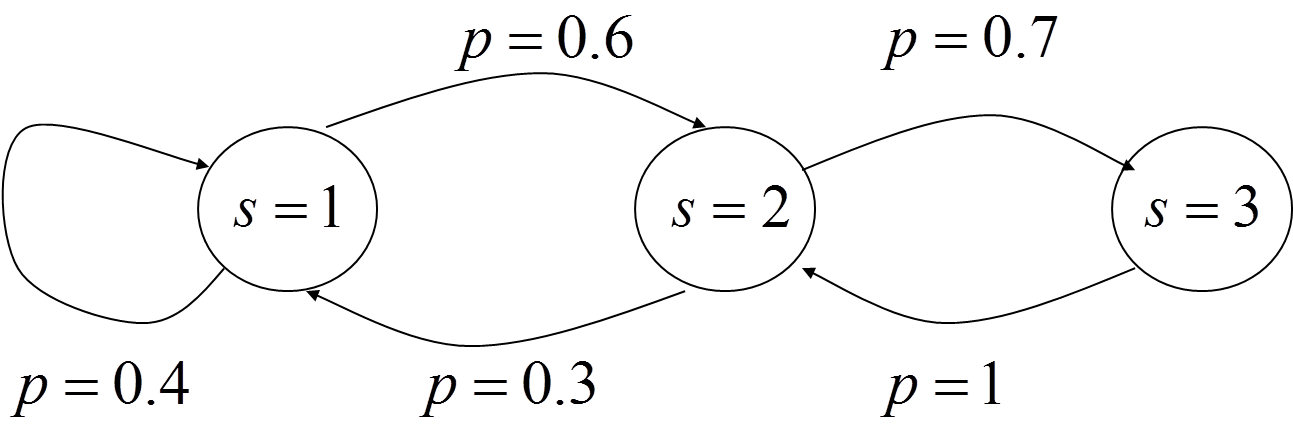
\includegraphics[width=0.7\textwidth]{lecture4_a}\\
  \caption{Markov chain}\label{fig:MC}
  \end{centering}
\end{figure}

A graphical description of a controlled Markov chain is a bit more complicated because of the additional action variable. We obtain the diagram (drawn for state $s = 1$ only, and for a given time $t$) in Figure \ref{fig:MDP}, reflecting the following transition probabilities:
\[\begin{array}{l}
p(s' = 2|s = 1,a = 1) = 1\\
p(s'|s = 1,a = 2) = \left\{ {\begin{array}{*{20}{c}}
{0.3}&:&{s' = 1}\\
{0.2}&:&{s' = 2}\\
{0.5}&:&{s' = 3}
\end{array}} \right.
\end{array}\]

\begin{figure}
  % Requires \usepackage{graphicx}
  \begin{centering}
  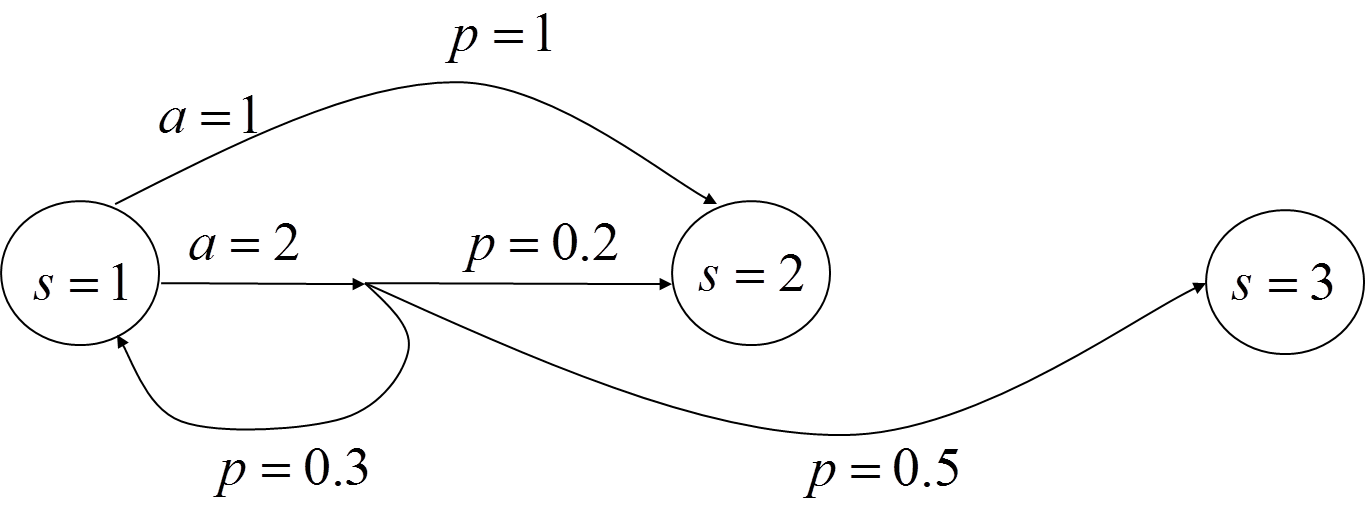
\includegraphics[width=0.7\textwidth]{lecture4_b}\\
  \caption{Controlled Markov chain}\label{fig:MDP}
  \end{centering}
\end{figure}


\paragraph{State-equation notation:}
The stochastic state dynamics can be equivalently defined in terms of a state equation of the form
                                                   \[{s_{t + 1}} = {f_t}({s_t},{a_t},{w_t}),\]
where ${w_t}$ is a random variable.
 	If  ${({w_t})_{t \ge 0}}$ is a sequence of independent RVs, and further each ${w_t}$ is independent of the "past"  $({s_{t - 1}},{a_{t - 1}}, \ldots, {s_0})$, then ${({s_t},{a_t})_{t \ge 0}}$ is a controlled Markov process.
 	For example, the state transition law of the last example can be written in this way, using
                  ${w_t} \in \{ 4,5,6\} $,  with  ${p_w}(4) = 0.3,\;{p_w}(5) = 0.2,\;{p_w}(6) = 0.5$
and, for ${s_t} = 1$:
    \[\begin{array}{l}
 	{f_t}(1,1,{w_t}) = 2\\
 	{f_t}(1,2,{w_t}) = {w_t} - 3
 	\end{array}.\]
The state equation notation is especially useful for problems with continuous state space, but also for some models with discrete states.


\paragraph{Control Policies}
\begin{itemize}
  \item A general or \textbf{history-dependent} control policy $\pi  = {({\pi _t})_{t \in {\bf{T}}}}$ is a mapping from each possible history ${h_t} = ({s_0},{a_0}, \ldots ,{s_{t - 1}},{a_{t - 1}},{s_t})$, $t \in {\bf{T}}$, to an action ${a_t} = {\pi _t}({h_t}) \in {A_t}$.  We denote the set of general policies by ${\Pi _G}$.
  \item A \textbf{Markov} control policy $\pi $ is allowed to depend on the current state and time only: ${a_t} = {\pi _t}({s_t})$.   We denote the set of Markov policies by ${\Pi _M}$.
  \item For stationary models, we may define \textbf{stationary} control policies that depend on the current state alone. A stationary policy is defined by a single mapping $\pi :S \to A$, so that  ${a_t} = \pi ({s_t})$ for all $t \in {\bf{T}}$. We denote the set of stationary policies by ${\Pi _S}$.
  \item Evidently, ${\Pi _G} \supset {\Pi _M} \supset {\Pi _S}$.
\end{itemize}

\paragraph{Randomized Control policies}
\begin{itemize}
  \item The control policies defined above specify deterministically the action to be taken at each stage. In some cases we want to allow for a random choice of action.
  \item A general randomized control policy assigns to each possible history ${h_t}$ a probability distribution ${\pi _t}( \cdot |{h_t})$ over the action set ${A_t}$. That is,  $prob\{ {a_t} = a|{h_t}\}  = {\pi _t}(a|{h_t})$. We denote the set of general randomized policies by ${\Pi _{GR}}$.
  \item Similarly, we can define the set ${\Pi _{MR}}$ of Markov randomized control policies, where ${\pi _t}( \cdot |{h_t})$ is replaced by ${\pi _t}( \cdot |{s_t})$, and the set ${\Pi _{SR}}$ of stationary randomized control policies, where ${\pi _t}( \cdot |{s_t})$ is replaced by  $\pi ( \cdot |{s_t})$.
  \item Note that the set ${\Pi _{GR}}$ includes all other policy sets as special cases.
\end{itemize}

\paragraph{The Induced Stochastic Process}
 	Let  ${p_0} = \{ {p_0}(s),s \in {S_0}\} $ be a probability distribution for the initial state ${s_0}$.
 	A control policy $\pi  \in {\Pi _{GR}}$, together with the transition law $P = \{ {p_t}(s'|s,a)\} $ and the initial state distribution ${p_0} = ({p_0}(s),\;s \in {S_0})$, induce a probability distribution over any finite state-action sequence  ${h_T} = ({s_0},{a_0}, \ldots ,{s_{T - 1}},{a_{T - 1}},{s_T})$, given by
\[P({h_T}) = {p_0}({s_0})\prod\limits_{t = 0}^{T - 1} {p({s_{t + 1}}|{s_t},{a_t}){\pi _t}({a_t}|{h_t})} .\]
To see this, observe the recursive relation:
                      \[\begin{array}{c}
P({h_{t + 1}}) = P({h_t},{a_t},{s_{t + 1}}) = P({s_{t + 1}}|{h_t},{a_t})P({a_t}|{h_t})P({h_t})\\
 = {p_t}({s_{t + 1}}|{s_t},{a_t}){\pi _t}({a_t}|{h_t})P({h_t}).
\end{array}\]
In the last step we used the conditional Markov property of the controlled chain: $P({s_{t + 1}}|{h_t},{a_t}) = {p_t}({s_{t + 1}}|{s_t},{a_t})$, and the definition of the control policy $\pi $.  The required formula follows by recursion.

Therefore, the state-action sequence ${h_\infty } = {({s_k},{a_k})_{k \ge 0}}$ can now be considered a stochastic process. We denote the probability law of this stochastic process by  ${P^{\pi ,{p_0}}}( \cdot )$. The corresponding expectation operator is denoted by ${E^{\pi ,{p_0}}}( \cdot )$.
When the initial state ${s_0}$ is deterministic (i.e., ${p_0}(s)$ is concentrated on a single state $s$), we may simply write ${P^{\pi ,s}}( \cdot )$  or ${P^\pi }( \cdot |{s_0} = s)$.

Under a Markov control policy, the state sequence ${({s_t})_{t \ge 0}}$ becomes a \emph{Markov chain}, with transition probabilities
                            \[P({s_{t + 1}} = s'|{s_t} = s) = \sum\nolimits_{a \in {A_t}} {{p_t}} (s'|s,a){\pi _t}(a|s).\]
\begin{exercise}{Prove this!}\end{exercise}

If the controlled Markov chain is stationary (time-invariant) and the control policy is stationary, then the induced Markov chain is stationary as well.



\begin{remark}
For most non-learning optimization problems, Markov policies suffice to achieve the optimum.
\end{remark}
\begin{remark}
Implicit in these definitions of control policies is the assumption that the current state ${s_t}$ can be fully observed before the action ${a_t}$ is chosen . If this is not the case we need to consider the problem of a Partially Observed MDP (POMDP), which is more involved.
\end{remark}

\section{Performance Criteria}

\subsection{Finite Horizon Problems}
Consider the finite-horizon problem, with a fixed time horizon $T$.
As in the deterministic case, we are given a running reward function ${r_t} = \{ {r_t}(s,a):s \in {S_t},a \in {A_t}\} $ for $0 \le t \le T - 1$, and a terminal reward function ${r_T} = \{ {r_T}(s):s \in {S_T}\} $.  The obtained rewards are then ${R_t} = {r_t}({s_t},{a_t})$ at times $t \le T - 1$, and ${R_T} = {r_T}({s_T})$ at the last stage.
Our general goal is to maximize the cumulative return:
                                             \[\sum\limits_{t = 0}^T {{R_t}}  = \sum\limits_{t = 0}^{T - 1} {{r_t}({s_t},{a_t}) + {r_T}({s_T})} .\]
However, since the system is stochastic, the cumulative return will generally be random, and we need to specify in which sense to maximize it.
A natural first option is to consider the expected value of the return. That is, define:
\[J_T^\pi (s) = {E^\pi }\left(\sum\limits_{t = 0}^T {{R_t}} |{s_0} = s\right) \equiv {E^{\pi ,s}}\left(\sum\limits_{t = 0}^T {{R_t}} \right)\]
 Here $\pi $ is the control policy as defined above, and $s$ denotes the initial state. Hence,  $J_T^\pi (s)$ is the expected cumulative return under the control policy $\pi $.  Our goal is to find an optimal control policy that maximizes $J_T^\pi (s)$.

\paragraph{Remarks:}
\begin{enumerate}
  \item Dependence on the next state:  In some problems, the obtained reward may depend on the next state as well: ${R_t} = {\tilde r_t}({s_t},{a_t},{s_{t + 1}})$.  For control purposes, when we only consider the expected value of the reward, we can reduce this reward function to the usual one by defining:
\[{r_t}(s,a) \buildrel \Delta \over = E({R_t}|{s_t} = s,{a_t} = a) \equiv \sum\nolimits_{s' \in S} {p(s'|s,a){{\tilde r}_t}(} s,a,s')\]
  \item Random rewards:  The reward ${R_t}$ may also be random, namely a random variable whose distribution depends on $({s_t},{a_t})$.  This can also be reduced to our standard model for planning purposes by looking at the expected value of ${R_t}$, namely \[{r_t}(s,a) = E({R_t}|{s_t} = s,{a_t} = a).\]
  \item Risk-sensitive criteria: The expected cumulative return is by far the most common goal for planning. However it is not the only one possible. For example, one may consider the following risk-sensitive  return function:
\[J_{_{T,\lambda }}^\pi (s) = \frac{1}{\lambda }\log {E^{\pi ,s}}(\exp (\lambda \sum\limits_{t = 0}^T {{R_t}} )).\]
For $\lambda  > 0$, the exponent gives higher weight to high rewards, and the opposite for $\lambda  < 0$.
\end{enumerate}

\subsection{Infinite Horizon Problems}
We next consider planning problems that extend to an unlimited time horizon, $t = 0,1,2, \ldots $. Such planning problems arise when the system in question is expected to operate for a long time, or a large number of steps, possibly with no specific "closing" time.
Infinite horizon problems are most often defined for stationary problems. In that case, they enjoy the important advantage that optimal policies can be found among the class of stationary policies.  We will restrict attention here to stationary models.
As before, we have the running reward function $r(s,a)$, which extends to all $t \ge 0$. The reward obtained at stage $t$ is  ${R_t} = r({s_t},{a_t})$.

\paragraph{Discounted return:} The most common performance criterion for infinite horizon problems is the expected discounted return:
\[J_\alpha ^\pi (s) = {E^\pi }\left(\sum\limits_{t = 0}^\infty  {{\alpha ^t}r({s_t},{a_t})} |{s_0} = s\right) \equiv {E^{\pi ,s}}\left(\sum\limits_{t = 0}^\infty  {{\alpha ^t}r({s_t},{a_t})} \right)\]
Here $0 < \alpha  < 1$ is the discount factor. Mathematically, the discount factor ensures convergence of the sum (whenever the reward sequence is bounded). This make the problem "well behaved", and relatively easy to analyze.
\paragraph{Average return:}  Here we are interested in maximizing the long-term average return. The most common definition of the long-term average return is
\[J_{av}^\pi (s) = \mathop {\lim \inf }\limits_{T \to \infty } {E^{\pi ,s}}\left(\frac{1}{T}\sum\limits_{t = 0}^{T - 1} {r({s_t},{a_t})} \right)\]
The theory of average-return planning problems is more involved, and relies to a larger extent on the theory of Markov chains.


\subsection{Stochastic Shortest-Path Problems}
In an important class of planning problems, the time horizon is not set beforehand, but rather the problem continues until a certain event occurs. This event can be defined as reaching some goal state.
Let  ${S_G} \subset S$ define the set of \emph{goal states}. Define
\[\tau  = \inf \{ t \ge 0:{s_t} \in {S_G}\} \]
as the first time in which a goal state is reached. The total expected return for this problem is defined as:
\[J_{ssp}^\pi (s) = {E^{\pi ,s}}\left(\sum\limits_{t = 0}^{\tau  - 1} {r({s_t},{a_t})}  + {r_G}({s_\tau })\right)\]
Here ${r_G}(s),\;s \in {S_G}$ specified the reward at goal states.

This class of problems provides a natural extension of the standard shortest-path problem to stochastic settings.  Some conditions on the system dynamics and reward function must be imposed for the problem to be well posed (e.g., that a goal state may be reached  with probability one).
Such problems are known as stochastic shortest path problems, or also episodic planning problems.

\section{*Sufficiency of Markov Policies}
In all the performance criteria defined above, the criterion is composed of sums of terms of the form $E({r_t}({s_t},{a_t}))$. It follows that if two control policies induce the same marginal probability distributions ${p_t}({s_t},{a_t})$ over the state-action pairs $({s_t},{a_t})$ for all $t \ge 0$, they will have the same performance.

Using this observation, the next claim implies that it is enough to consider the set of (randomized) Markov policies in the above planning problems.

\begin{proposition}\label{prop:sufficient} Let  $\pi  \in {\Pi _{GR}}$ be a general (history-dependent, randomized) control policy.  Let
\[p_t^{\pi ,{s_0}}(s,a) = {P^{\pi ,{s_0}}}({s_t} = s,{a_t} = a),\quad \;\;(s,a) \in {S_t} \times {A_t}\]
Denote the marginal distributions induced by $({s_t},{a_t})$ on the state-action pairs $({s_t},{a_t})$, for all $t \ge 0$.
Then there exists a randomized Markov policy $\tilde \pi $ that induces the same marginal probabilities (for all initial states ${s_0}$).
\end{proposition}
\begin{exercise}[\textbf{Challenge Problem 1}] Prove Proposition \ref{prop:sufficient}.

Note: If you consult a reference or a friend, mention that in your solution.
\end{exercise}


\section{Finite-Horizon Dynamic Programming}

Recall that we consider the expected total reward criterion, which we denote as
\[{J^\pi }({s_0}) = {E^{\pi ,{s_0}}}\left( {\sum\nolimits_{t = 0}^{T - 1} {{r_t}({s_t},{a_t}) + {r_T}({s_T})} } \right)\]
Here $\pi $ is the control policy used, and ${s_0}$ is a given initial state. We wish to maximize ${J^\pi }({s_0})$ over all control policies, and find an optimal policy ${\pi ^*}$ that achieves the maximal reward ${J^*}({s_0})$ for all initial states ${s_0}$.  Thus,
\[{J^*}({s_0}) \buildrel \Delta \over = {J^{\pi *}}({s_0}) = \mathop {\max }\limits_{\pi  \in {\Pi _{GR}}} {J^\pi }({s_0})\]


\subsection{The Principle of Optimality}
The celebrated principle of optimality (stated by Bellman) applies to a large class of multi-stage optimization problems, and is at the heart of DP. As a general principle, it states that:
\begin{center}
\textbf{The tail of an optimal policy is optimal for the "tail" problem.}
\end{center}

This principle is not an actual claim, but rather a guiding principle that can be applied in different ways to each problem.
For example, considering our finite-horizon problem, let ${\pi ^*} = ({\pi _0}, \ldots ,{\pi _{T - 1}})$ denote an optimal Markov policy. Take any state ${s_t} = s'$ which has a positive probability to be reached under ${\pi ^*}$, namely ${P^{\pi^* ,{s_0}}}({s_t} = s') > 0$. Then the tail policy $({\pi _t}, \ldots ,{\pi _{T - 1}})$ is optimal for the "tail" criterion $J_{t:T}^\pi (s') = {E^\pi }\left( {\sum\nolimits_{k = t}^T {{R_k}|{s_t} = s'} } \right)$.


\subsection{Dynamic Programming for Policy Evaluation}\label{sss:pol_eval}
As a "warmup", let us evaluate the reward of a given policy.
Let $\pi  = ({\pi _0}, \ldots ,{\pi _{T - 1}})$ be a given Markov policy. Define the following reward-to-go function, or value function:
\[V_k^\pi (s) = {E^\pi }\left( {\sum\nolimits_{t = k}^T {{R_t}|{s_k} = s} } \right)\]
Observe that $V_0^\pi ({s_0}) = {J^\pi }({s_0})$.

\begin{lemma}[\textbf{Value Iteration}]\label{lem:finite_horizon_VI} $V_k^\pi (s)$ may be computed by the backward recursion:
\[V_k^\pi (s) = {\left\{ {{r_k}(s,a) + \sum\nolimits_{s' \in {S_{k + 1}}} {{p_k}(s'|s,a)} \;V_{k + 1}^\pi (s')} \right\}_{a = {\pi _k}(s)}}\;,\quad s \in {S_k}\]
for $k =  T - 1, \ldots ,0 $,  starting with  $V_T^\pi (s) = {r_T}(s)$.
\end{lemma}
\begin{proof}
Observe that:
\begin{align*}
V_k^\pi (s) &= {E^\pi }\left( {{R_k} + \sum\nolimits_{t = k + 1}^N {{R_t}|} \;{s_k} = s,{a_k} = {\pi _k}(s)} \right)\\
 &= {E^\pi }\left( {{E^\pi }\left( {{R_k} + \sum\nolimits_{t = k + 1}^N {{R_t}} |\;{s_k} = s,{a_k} = {\pi _k}(s),{s_{k + 1}}} \right)|{s_k} = s,{a_k} = {\pi _k}(s)} \right)\\
 &= {E^\pi }\left( {r({s_k},{a_k}) + V_{k + 1}^\pi ({s_{k + 1}})|{s_k} = s,{a_k} = {\pi _k}(s)} \right)\\
 &= {r_k}(s,{\pi _k}(s)) + \sum\nolimits_{s' \in {S_{k + 1}}} {{p_k}(s'|s,{\pi _k}(s))} \;V_{k + 1}^\pi (s')
\end{align*}
\end{proof}
\paragraph{Remarks:}
\begin{itemize}
  \item Note that $\sum\nolimits_{s' \in {S_{k + 1}}} {{p_k}(s'|s,a)} \;V_{k + 1}^\pi (s') = {E^\pi }(V_{k + 1}^\pi ({s_{k + 1}})|{s_k} = s,{a_k} = a)$.
  \item For the more general reward function ${\tilde r_t}(s,a,s')$, the recursion takes the form
                     \[V_k^\pi (s) = {\left\{ {\sum\nolimits_{s' \in {S_{k + 1}}} {{p_k}(s'|s,a)} [{r_k}(s,a,s') + V_{k + 1}^\pi (s')]} \right\}_{a = {\pi _k}(s)}}\]
A similar observation applies to all Dynamic Programming equations below.
\end{itemize}

\subsection{Dynamic Programming for Policy Optimization}

We next define the optimal value function at each time $k \ge 0$ :
\[V_k^{}(s) = \mathop {\max }\limits_{{\pi ^k}} {E^{{\pi ^k}}}\left( {\sum\nolimits_{t = k}^T {{R_t}|{s_k} = s} } \right),\quad \,s \in {S_k}\]
The maximum is taken over "tail" policies ${\pi ^k} = ({\pi _k}, \ldots ,{\pi _{T - 1}})$ that start from time $k$. Note that ${\pi ^k}$ is allowed to be a general policy, i.e., history-dependent and randomized.
Obviously, ${V_0}({s_0}) = {J^*}({s_0})$.

\begin{theorem}[\textbf{Finite-horizon Dynamic Programming}]\label{thm:finite_horizon_DP}
The following holds:
\begin{enumerate}
\item Backward recursion:  Set $V_T^{}(s) = {r_T}(s)$ for $s \in {S_T}$.\\
     For $k = T - 1, \ldots ,0$, $V_k^{}(s)$ may be computed using the following recursion:
\[V_k^{}(s) = \mathop {\max }\limits_{a \in {A_k}} \left\{ {{r_k}(s,a) + \sum\nolimits_{s' \in {S_{k + 1}}} {{p_k}(s'|s,a)\,} V_{k + 1}^{}(s')} \right\},  \quad  s \in {S_k}.\]
\item Optimal policy: Any Markov policy ${\pi ^*}$ that satisfies, for $t = 0, \ldots ,T - 1$,
\[\pi _t^*(s) \in \mathop {\arg \max }\limits_{a \in {A_t}} \left\{ {{r_t}(s,a) + \sum\nolimits_{s' \in {S_{t + 1}}} {{p_t}(s'|s,a)\,} V_{t + 1}^{}(s')} \right\},\quad s \in {S_t},\]
is an optimal control policy. Furthermore, ${\pi ^*}$ maximizes ${J^\pi }({s_0})$ simultaneously
for every initial state ${s_0} \in {S_0}.$
\end{enumerate}
\end{theorem}
Note that Theorem \ref{thm:finite_horizon_DP} specifies an optimal control policy which is a deterministic Markov policy.

\begin{proof}
\textbf{Part (i):}

We use induction to show that the stated backward recursion indeed yields the optimal value function. The idea is simple, but some care is needed with the notation since we consider general policies, and not just Markov policies.
The equality $V_T^{}(s) = {r_T}(s)$ follows directly from the definition of $V_T^{}$.

We proceed by backward induction. Suppose that $V_{k + 1}^{}(s)$ is the optimal value function for time $k + 1$. We need to show that $V_k^{}(s) = {W_k}(s)$, where
                       \[{W_k}(s) \buildrel \Delta \over = {\max _{a \in {A_k}}}\left\{ {{r_k}(s,a) + \sum\nolimits_{s' \in {S_{k + 1}}} {{p_k}(s'|s,a)\,} V_{k + 1}^{}(s')} \right\}.\]
We will first establish that $V_k^{}(s) \ge {W_k}(s)$, and then that $V_k^{}(s) \le {W_k}(s)$.

(a) We first show that $V_k^{}(s) \ge {W_k}(s)$. For that purpose, it is enough to find a policy ${\pi ^k}$ so that $V_k^{{\pi ^k}}(s) = {W_k}(s)$.

Fix $s \in {S_k}$, and define ${\pi ^k}$ as follows: Choose ${a_k} = \bar a$, where
\[\bar a \in \mathop {\arg \max }\limits_{a \in {A_k}} \left\{ {{r_k}(s,a) + \sum\nolimits_{s' \in {S_{k + 1}}} {{p_k}(s'|s,a)} \,V_{k + 1}^{}(s')} \right\},\]
and then, after observing  ${s_{k + 1}} = s'$, proceed with the optimal tail policy ${\pi ^{k + 1}}(s')$ that obtains $V_{k + 1}^{{\pi ^{k + 1}}(s')}(s') = {V_{k + 1}}(s')$. Proceeding similarly to Subsection \ref{sss:pol_eval} above (value iteration for a fixed policy), we obtain:
\begin{align}
V_k^{{\pi ^k}}(s) &= {r_k}(s,\bar a) + \sum\nolimits_{s' \in {S_{k + 1}}} {p(s'|s,\bar a)\,} V_{k + 1}^{{\pi ^{k + 1}}(s')}(s')\\
 &= {r_k}(s,\bar a) + \sum\nolimits_{s' \in {S_{k + 1}}} {p(s'|s,\bar a)} \,V_{k + 1}^{}(s') = {W_k}(s),
\end{align}
as was required.

(b) To establish $V_k^{}(s) \le {W_k}(s)$, it is enough to show that $V_k^{{\pi ^k}}(s) \le {W_k}(s)$ for any (general, randomized) "tail" policy ${\pi ^k}$.

Fix $s \in {S_k}$.
Consider then some tail policy ${\pi ^k} = ({\pi _k}, \ldots {\pi _{T - 1}})$. Note that this means that ${a_t} \sim {\pi _t}(a|{h_{k:t}})$, where ${h_{k:t}} = ({s_k},{a_k},{s_{k + 1}},{a_{k + 1}}, \ldots ,{s_t})$. For each state-action pair $s \in {S_k}$ and $a \in {A_k}$, let  $({\pi ^k}|s,a)$ denote the tail policy ${\pi ^{k + 1}}$ from time $k + 1$ onwards which is obtained from ${\pi ^k}$ given that ${s_k} = s,\;{a_k} = a$. As before, by value iteration for a fixed policy,
\[V_k^{{\pi ^k}}(s) = \sum\nolimits_{a \in {A_k}} {{\pi _k}(a|s)\left\{ {{r_k}(s,a) + \sum\nolimits_{s' \in {S_{k + 1}}} {{p_k}(s'|s,a)} \,V_{k + 1}^{({\pi ^k}|s,a)}(s')} \right\}} .\]
But since $V_{k + 1}^{}$ is optimal,
\begin{align*}
V_k^{{\pi ^k}}(s) &\le \sum\nolimits_{a \in {A_k}} {{\pi _k}(a|s)\left\{ {{r_k}(s,a) + \sum\nolimits_{s' \in {S_{k + 1}}} {{p_k}(s'|s,a)\,} V_{k + 1}^{}(s')} \right\}} \\
 &\le {\max _{a \in {A_k}}}\left\{ {{r_k}(s,a) + \sum\nolimits_{s' \in {S_{k + 1}}} {{p_k}(s'|s,a)\,} V_{k + 1}^{}(s')} \right\} = {W_k}(s),
\end{align*}
which is the required inequality in (b).

\textbf{Part  (ii)} (Outline - \textbf{exercise}):

Let ${\pi ^*}$ be the (Markov) policy defined in part 2 of Theorem \ref{thm:finite_horizon_DP}. Using value iteration for this policy, prove by backward induction that $V_k^{{\pi ^*}} = V_k^{}$.
\end{proof}

\paragraph{To summarize:}
\begin{itemize}
  \item The optimal value function can be computed by backward recursion. This recursive equation is known as the \emph{dynamic programming equation}, \emph{optimality equation}, or \emph{Bellman's Equation}.
  \item Computation of the value function in this way is known as the \emph{finite-horizon value iteration} algorithm.
  \item The value function is computed for all states at each stage.
  \item An optimal policy is easily derived from the optimal value.
  \item The optimization in each stage is performed in the action space.  The total number of minimization operations needed is $T \times |S|$  - each over $|A|$ choices. This replaces "brute force" optimization in policy space, with tremendous computational savings as the number of Markov policies is $|A{|^{T\times |S|}}$.
\end{itemize}

\subsection{The Q function}
Let
\[{Q_k}(s,a) \buildrel \Delta \over = {r_k}(s,a) + \sum\nolimits_{s' \in {S_{k+1}}} {{p_k}(s'|s,a)\,V_{k+1}^{}(s')} .\]
This is known as the optimal state-action value function, or simply as the \emph{Q-function}. ${Q_k}(s,a)$ is the expected return from stage $k$ onward, if we choose ${a_k} = a$  and then proceed optimally.

Theorem \ref{thm:finite_horizon_DP} can now be succinctly expressed as
\[V_k^{}(s) = \mathop {\max }\limits_{a \in {A_k}} {Q_k}(s,a),\]
and
\[\pi _k^*(s) \in \mathop {\arg \max }\limits_{a \in {A_k}} {Q_k}(s,a).\]
The Q function provides the basis for the Q-learning algorithm, which is one of the basic Reinforcement Learning algorithms.



